\subsection{Consideraciones generales}
Para armar los circuitos propuestos por la cátedra se dispone de un
amplificador operacional LM-833N. Los datos más importantes a considerar
vistos en la hoja de datos son los siguientes:
\begin{enumerate}
    \item $A_{vol}$ = $110dB$
    \item BWP = $15 MHz$

\end{enumerate}    

\subsection{Circuito Derivador}
A continuación se realiza el análisis sobre el circuito derivador planteado
por la cátedra utilzando un amplificador operancional $LM833$ propuestado por 
la cátedra en el siguiente circuito.
\begin{figure}[H]
    \centering
    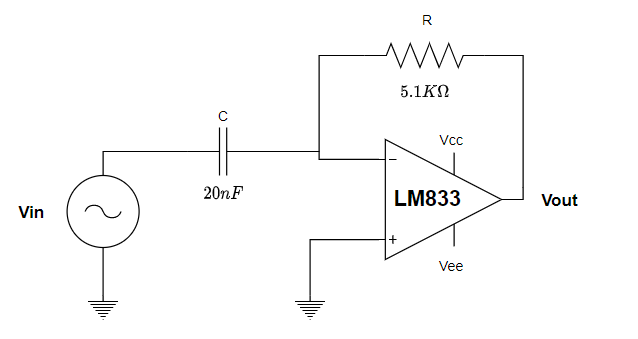
\includegraphics[width=0.6\textwidth]{../Ejercicio3-CircuitoIntegradoresyDerivadores/Imagenes/Derivador/circuito_derivador.png}
    \caption{Circuito derivador implementado con Opamp}
\end{figure}

Consiguientemente, se procede a calcular la transferencia de tensión entra
la entrada y salida del circuito. \par 
En condición ideales se puede se considera que la ganancia del
amplificador operacional es infinita por lo que, basándonos en 
su ecuación característica (\ref{eq_opamp}), se puede asegurar que para 
mantener la relación $V^+=V^-$ van a tender a 0.
\vspace{2mm}
\begin{equation*}
    V_{out}=A_0(V^+-V^-)
    \label{eq_opamp}
\end{equation*}
\vspace{2mm}
Por lo tanto, se pueden escribir a las corrientes del circuito como:
\vspace{2mm}
\begin{equation*}
    I_1=\frac{V{in}}{X_c}=V_{in}\$C_1 \indent \indent I_2=\frac{V_{out}}{R}
    \label{eq_avol_ideal}
\end{equation*}
\vspace{2mm}
Considerando que $V^-=0$ y que $I_1=I_2$ se logra llegar a la transferencia bajo 
condiciones ideales:
\vspace{2mm}
\begin{equation}
    H(\$)=\frac{V_{out}}{V_{in}}=-R\$C
    \label{trans_ideal}
\end{equation}
\vspace{2mm}
Por otro lado, considerando a $A_{vol}$ finito se vuelve indispensable reformular las
ecuaciones vistas en \ref{eq_avol_ideal} ya que al considerar un $A_vol$ que no 
tiende a infinito se vuelve imposible asegurar que la tensión $V^-$ sea nula. Bajo 
las nuevas circunstancias se obtienen:
\vspace{2mm}
\begin{equation*}
    I_1=\frac{V{in}-V^-}{X_c}=(V_{in}-V^-)\$C_1 \indent \indent I_2=\frac{V_{out}-V^-}{R}
    \label{eq_avol_noideal}
\end{equation*}
\vspace{2mm}
Utilizando \ref{eq_opamp} y \ref{eq_avol_noideal} se puede despejar la transferencia
como:
\vspace{2mm}
\begin{equation}
    H_1(\$)=\frac{V_{out}}{V_{in}}=\frac{-R\$C}{1+(\frac{R\$C+1}{A_0})}
    \label{trans_no_ideal}
\end{equation}
\vspace{2mm}
Se puede validar este ecuación considerando:
 $$\lim_{A_0\to\infty} H_1(\$)$$
Se obtiene la transferencia en condiciones ideales vista en \ref{trans_ideal}. \par
Para finalizar se realiza un análisis considerando $A_{vol}$ variante en frecuencia
debido a la presencia de un polo dominante que le da una respuesta en frecuencia 
característica de un filtro pasa-bajos. La dependencia en frecuencia de la ganancia
del opamp está dada por la siguiente fórmula:
\vspace{2mm}
\begin{equation}
    A_v(\$)=\frac{A_0}{1+\frac{\$}{w_b}}
    \label{a_vol_frec}
\end{equation}
\vspace{2mm}
Siendo $A_0$ la ganancia en continua y $w_b$ el ancho de banda del filtro,
 la frecuencia para la cual el dispositivo atenúa 3 dB. \par 
 Reemplazando (\ref{a_vol_frec}) en (\ref{trans_no_ideal}) se obtiene:
 \vspace{2mm}
 \begin{equation}
    H_2(\$)=\frac{-R\$C}{1+\frac{1}{A_0}+\frac{R\$C}{A_0}+\frac{R\$^2C}{w_bA_0}}
    \label{trans_frec}
\end{equation}
\vspace{2mm}
Esta ecuación se puede dividir según su ganancia ideal $G_I$ y su factor de corrección
$F_c$ de la siguiente forma:
\vspace{2mm}
\begin{equation*}
   G_I=-R\$C \indent \indent F_c=\frac{1}{1+\frac{1}{A_0}+\frac{R\$C}{A_0}+\frac{R\$^2C}{w_bA_0}}
   \label{trans_frec}
\end{equation*}
\vspace{2mm}
Siguiendo el mismo procedimiento aplicado para $H_1(\$)$, se puede 
 $$\lim_{A_0\to\infty} H_2(\$)=\lim_{A_0\to\infty} G_IF_C=G_I=H(\$)$$

Las expresiones obtenidas se plasman en el siguiente gráfico, pudiéndose 
observar una mayor precisión a medida que se usan modelos más realistas
sin consideraciones ideales.
\begin{figure}[H]
    \centering
    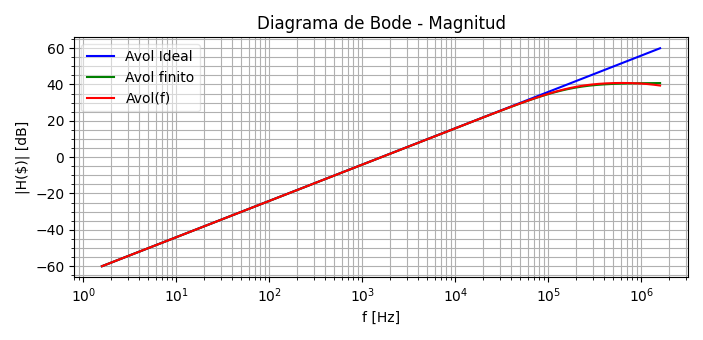
\includegraphics[width=0.6\textwidth]{../Ejercicio3-CircuitoIntegradoresyDerivadores/Imagenes/Derivador/bode_derivador magnitud.png}
    \caption{Respuesta en frecuencia teóricas - Modulo}
\end{figure}
\begin{figure}[H]
    \centering
    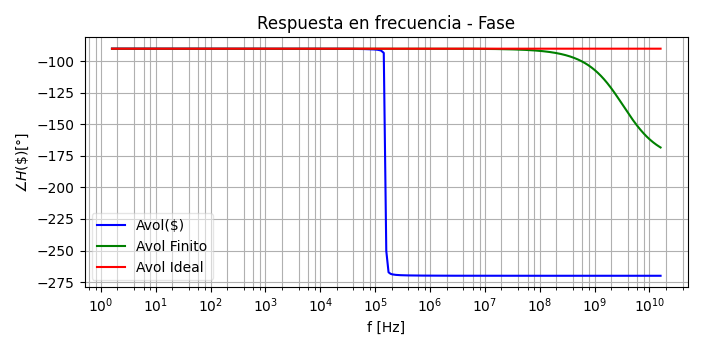
\includegraphics[width=0.6\textwidth]{../Ejercicio3-CircuitoIntegradoresyDerivadores/Imagenes/Derivador/bode_derivador_fase.png}
    \caption{Respuesta en frecuencia teóricas - Fase}
\end{figure}












\subsection{Circuito Integrador}

\subsubsection{Introducción}

Se realizó el análisis de un circuito integrador ideal, utilizando en este caso los tres mismos componentes que para el integrador, una Resistencia $R$,
un capacitor $C$ y un amplificador operacional. 
Cabe destacar que se considera  a este circuito como un integrador ya que a diferencia del circuito RC analizado en el primer trabajo práctico de laboratorio,
éste funcionará como integrador "teórico" para cualquier frecuencia y no solo a frecuencias altas. 

Los valores nominales utilizados para la experiencia fueron:

\begin{itemize}
	\item $R: 5.1K \Omega$ 
	\item $C: 20nF$
	\item $OPAMP: LM833$
\end{itemize}

\begin{figure}[H]
    \centering 
    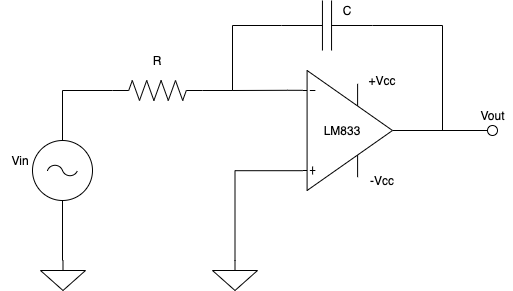
\includegraphics [scale=0.5] {../Ejercicio3-CircuitoIntegradoresyDerivadores/Imagenes/diagrama-integrador.png} 
    \caption{Diagrama del circuito integrador ideal empleado}
    \label{fig:emptyPlotTool}
\end{figure}

A continuación se procederá a calcular teóricamente el valor de las funciones transferencia para los casos en 
donde el amplificador operacional tiene un comportamiento ideal, con $A_{vol}$ finito y $A_{vol}(w)$ con polo dominante.

\subsubsection{Análisis de la Transferencia del Circuito Integrador - OPAMP ideal}

Para obtener la función transferencia en este caso, $H(S) = \frac{V_{out} (S)}{V_{in} (S)}$, partiremos de las siguientes condiciones
iniciales para el amplificador operacional:

\begin{itemize}
	\item $A_{vol}: \infty$
	\item $Z_{in}: \infty$
	\item $Z_{out}: 0$
\end{itemize}

\begin{figure}[H]
    \centering 
    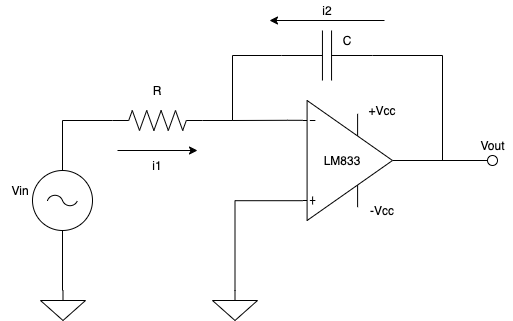
\includegraphics [scale=0.5] {../Ejercicio3-CircuitoIntegradoresyDerivadores/Imagenes/diagrama-integrador-corrientes.png} 
    \caption{Diagrama del circuito integrador ideal empleado}
    \label{fig:emptyPlotTool}
\end{figure}

Podemos observar a simple vista que:

\begin{itemize}
	\item $i1 = -i2$
	\item $i1 = \frac {V_{in}-V^{-}}{R} $
	\item $i2 = \frac {V_{out}-V^{-}}{X_c}$
	\item $V_{out} = A_{vol}(V^{+}-V^{-})$
\end{itemize}

Como ${A_{vol} \to \infty}$ y $V_{out}$ es finito, ${(V^{+}-V^{-}) \to 0}$ y como $V^{+}$ está conectado a tierra,
$V^{-}$ representa tierra virtual, por lo cual su valor es de $0V$.

Entonces, redefiniendo las ecuaciones anteriores:

\begin{itemize}
	\item $i1 = \frac{V_{in}}{R} $
	\item $i2 = \frac {V_{out}}{X_c}$
\end{itemize}

Siendo entonces:

$$ \frac{V_{in}}{R} = - (\frac{V_{out}}{X_c}) \Longrightarrow \frac{V_{out}}{V_{in}} = -\frac{X_c}{R} = - \frac{1}{SRC}$$

$$ H(S) = - \frac{1}{SRC}$$

Como se ha mencionado anteriormente, queda demostrado el comportamiento del sistema como integrador, ya que si antitransformamos la función de transferencia
obtenida implicará que para obtener $v_{out}(t)$ habrá que integrar $v_{in}(t)$ en el dominio del tiempo por tener el factor en el dominio de Laplace de $L(S)=\frac{1}{S}$

\begin{figure}[H]
    \centering 
    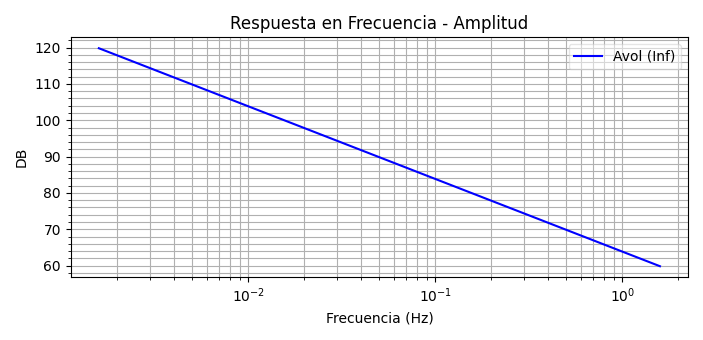
\includegraphics [scale=1] {../Ejercicio3-CircuitoIntegradoresyDerivadores/Imagenes/teorico-avol-inf-integrador-amplitud.png} 
    \caption{Respuesta en Frecuencia - Amplitud para OPAMP ideal}
    \label{fig:emptyPlotTool}
\end{figure}

\begin{figure}[H]
    \centering 
    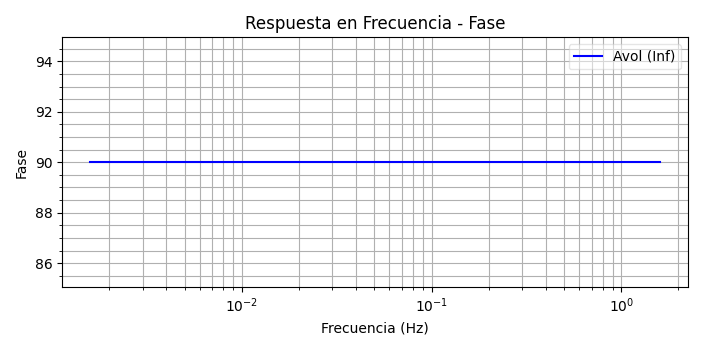
\includegraphics [scale=1] {../Ejercicio3-CircuitoIntegradoresyDerivadores/Imagenes/teorico-avol-inf-integrador-fase.png} 
    \caption{Respuesta en Frecuencia - Fase para OPAMP ideal}
    \label{fig:emptyPlotTool}
\end{figure}

\subsubsection{Análisis de la Transferencia del Circuito Integrador - OPAMP con $A_{vol}$ finito}

A diferencia del caso anterior, para el cálculo de la función transferencia, $H(S) = \frac{V_{out} (S)}{V_{in} (S)}$, partiremos de las condiciones planteadas previamente, excepto
:

\begin{itemize}
	\item $A_{vol}: finito$
\end{itemize}

Utilizando entonces las mismas relaciones, se puede observar ahora que:


$$V_{out}=-A_{vol}.V^{-} \Longrightarrow V^{-} = \frac{-V_{out}}{A_{vol}}$$ 


Por lo tanto:

\begin{itemize}
	\item $i1 = \frac {V_{in}-V^{-}}{R} =  \frac {V_{in} + \frac{V_{out}}{A_{vol}}}{R}$
	\item $i2 = \frac {V_{out}-V^{-}}{X_c} = \frac {V_{out} + \frac{V_{out}}{A_{vol}}}{X_c}$
\end{itemize}

Siendo entonces:

$$ \frac {V_{in} + \frac{V_{out}}{A_{vol}}}{R} = -(\frac {V_{out} + \frac{V_{out}}{A_{vol}}}{X_c})
\Longrightarrow \frac{V_{out}}{V_{in}} = \frac{-1}{SCR(1+\frac{1}{A_{vol}}+\frac{1}{A_{vol}SRC})} = \frac{-1}{SCR(1+\frac{1}{A_{vol}})+\frac{1}{A_{vol}}}$$

Finalmente:

$$H(S)= \frac{-A_{vol}}{SCR(A_{vol}+1)+1}$$

Es importante notar que siendo la ganancia para el caso ideal, donde $A_{vol}$ es $\infty$, $ GI = - \frac{1}{SRC}$,  la función
transferencia se puede representar como $H(S) = GI. \frac{-A_{vol}}{SCR(A_{vol}+1)+1}$. Y
si $A_{vol}$ es lo suficientemente grande, tendremos la función transferencia ideal nuevamente del primer caso analizado para el circuito integrador.

\begin{figure}[H]
    \centering 
    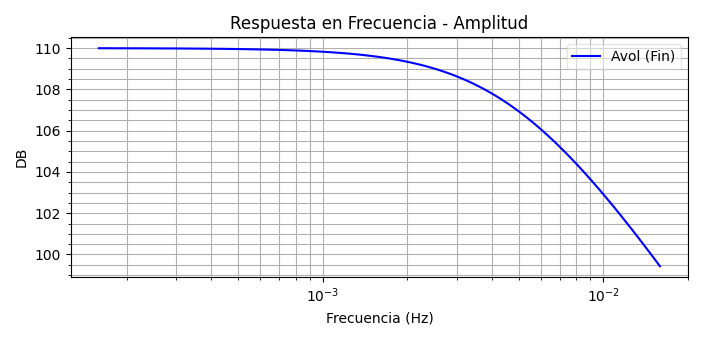
\includegraphics [scale=1] {../Ejercicio3-CircuitoIntegradoresyDerivadores/Imagenes/teorico-avol-fin-integrador-amplitud.png} 
    \caption{Respuesta en Frecuencia - Amplitud para OPAMP con $A_{vol}$ finito}
    \label{fig:emptyPlotTool}
\end{figure}

\begin{figure}[H]
    \centering 
    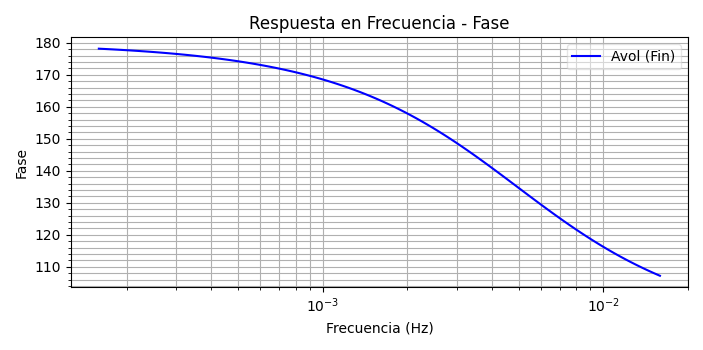
\includegraphics [scale=1] {../Ejercicio3-CircuitoIntegradoresyDerivadores/Imagenes/teorico-avol-fin-integrador-fase.png} 
    \caption{Respuesta en Frecuencia - Fase para OPAMP con $A_{vol}$ finito}
    \label{fig:emptyPlotTool}
\end{figure}

\subsubsection{Análisis de la Transferencia del Circuito Integrador - OPAMP con $A_{vol}(w)$}

En este último caso de analisis, $A_{vol}$ no es constante sino que es función de la frecuencia según:

$$A_{vol}(S)=\frac{A_0}{1+\frac{S}{w_b}}$$

Por lo cual la expresión para la función transferencia calculada en el caso anterior, quedará denominada por:

$$H(S)= \frac{-1}{SCR(1+\frac{1+\frac{1}{SCR}}{A_{vol}})}\Longrightarrow H(S)= \frac{-1}{SCR(1+\frac{1+\frac{1}{SCR}}{\frac{A_0}{1+\frac{S}{w_b}}})}$$ 

Reacomodando algebraicamente:

$$H(S)=- \frac{1}{S^2\frac{CR}{A_oW_b}+SCR(1 + \frac{1}{A_o}+\frac{1}{W_bA_oCR}) + \frac{1}{A_0}}$$

Finalmente:

$$H(S)=- \frac{{A_0}}{S^2\frac{CR}{W_b}+SCR({A_0} + 1+\frac{1}{W_bCR}) + 1 }$$

Podemos observar que si $A_o$ es muy grande, nuevamente estaremos en el caso donde la ganancia que obtendremos será la ideal para este circuito.

\begin{figure}[H]
    \centering 
    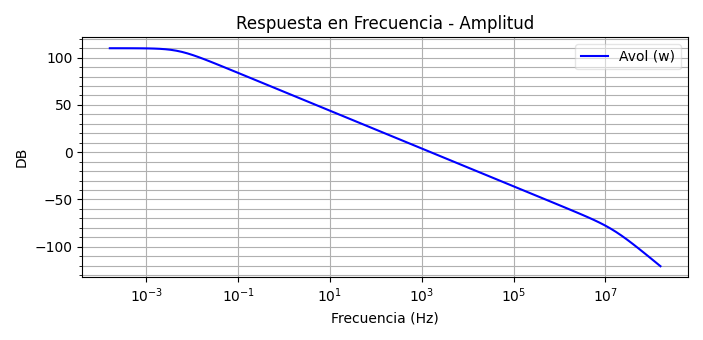
\includegraphics [scale=1] {../Ejercicio3-CircuitoIntegradoresyDerivadores/Imagenes/teorico-avol-w-integrador-amplitud.png} 
    \caption{Respuesta en Frecuencia - Amplitud para OPAMP con $A_{vol}(w)$}
    \label{fig:emptyPlotTool}
\end{figure}

\begin{figure}[H]
    \centering 
    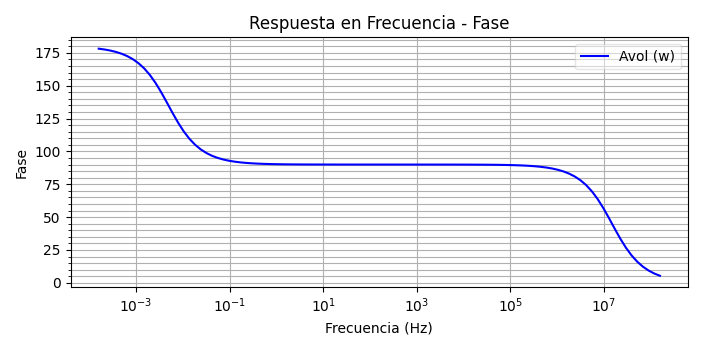
\includegraphics [scale=1] {../Ejercicio3-CircuitoIntegradoresyDerivadores/Imagenes/teorico-avol-w-integrador-fase.png} 
    \caption{Respuesta en Frecuencia - Fase para OPAMP con $A_{vol}(w)$ }
    \label{fig:emptyPlotTool}
\end{figure}

Comparando los tres casos, podemos observar que en determinado rango de frecuencias el comportamiento entre los tres casos es muy similar:

%%%%%%
%AGREGAR NUEVOS DIAGRAMAS COMPARATIVOS%

\begin{figure}[H]
    \centering 
    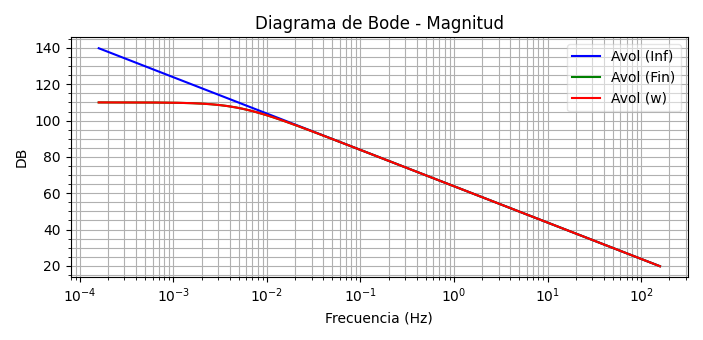
\includegraphics [scale=1] {../Ejercicio3-CircuitoIntegradoresyDerivadores/Imagenes/comparativo-magnitud.png} 
    \caption{Diagrama de BODE de Amplitud para OPAMP comparativo }
    \label{fig:emptyPlotTool}
\end{figure}

\begin{figure}[H]
    \centering 
    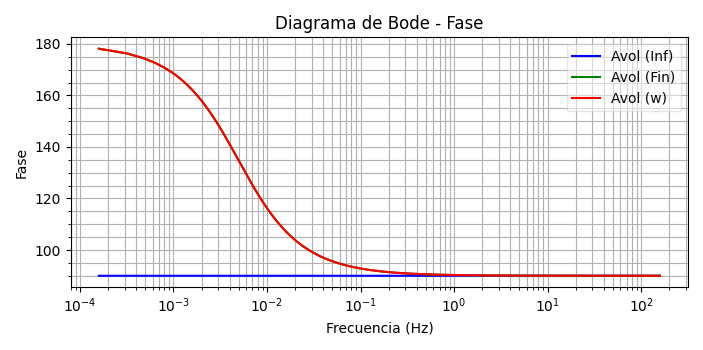
\includegraphics [scale=1] {../Ejercicio3-CircuitoIntegradoresyDerivadores/Imagenes/comparativo-fase.png} 
    \caption{Diagrama de BODE de Fase para OPAMP comparativo }
    \label{fig:emptyPlotTool}
\end{figure}

Gráficamente se puede observar que en el orden del $100 mHz$, los tres casos empiezan a comportarse de manera similar, tanto en su Respuesta en Frecuencia para la Amplitud
como para la Fase. Para el caso en el que $A_{vol}(w)$, observamos el efecto del polo dominante del amplificador operacional en el abrupto cambio de la fase. Para los cálculos de la presente sección y análizando
el DataSheet del amplificador operacional $LM833$, se obtubieron los siguientes valores:

\begin{itemize}
	\item $w_b = 298.011$
	\item $A_0 = 110 Db$
\end{itemize}

Además, como se está analizando el comportamiento del circuito como analizador y el comportamiento esperado no será ideal, se puede confirmar con solo observar los gráficos anteriores de 
Respuesta en Frecuencia, en especial, el comparativo entre los tres casos, que el rango real de frecuencias esperado, donde el circuito se comportará como ideal, será en donde la respuesta en frecuencia
para los tres casos, coincide.

Para aportar un valor adicional al análisis y contrastar lo obtenido teóricamente, se realizó la simulación correspondiente en el software $LTSpice$. Lo obtenido para la respuesta en frecuencia con los elementos
mencionados previamente es:

\begin{figure}[H]
    \centering 
    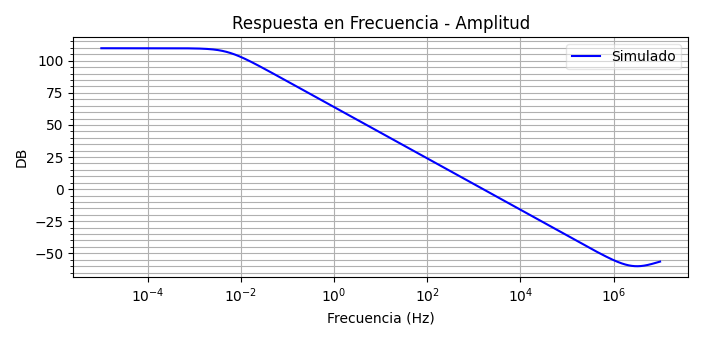
\includegraphics [scale=1] {../Ejercicio3-CircuitoIntegradoresyDerivadores/Imagenes/simulado-integrador-amplitud.png} 
    \caption{Respuesta en Frecuencia Simulada para Circuito Integrador - Amplitud }
    \label{fig:emptyPlotTool}
\end{figure}

\begin{figure}[H]
    \centering 
    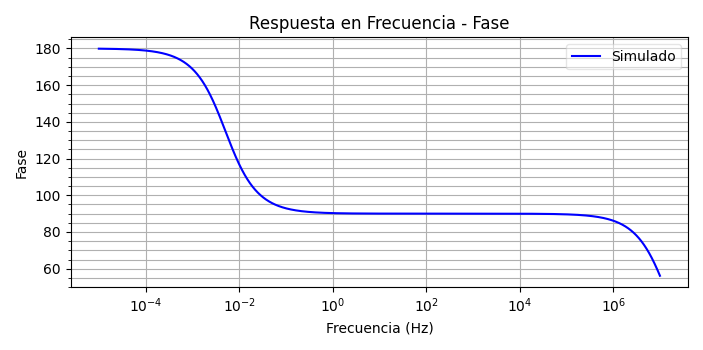
\includegraphics [scale=1] {../Ejercicio3-CircuitoIntegradoresyDerivadores/Imagenes/simulado-integrador-fase.png} 
    \caption{Respuesta en Frecuencia Simulada para Circuito Integrador - Fase }
    \label{fig:emptyPlotTool}
\end{figure}

Se puede observar que los resultados de la simulación muestran total similitud con lo analizado teóricamente para el caso $A_{vol}(w)$.

\subsubsection{Análisis de Entrada Senoidal al circuito integrador}

Se inyectó una señal senoidal variando su amplitud y frecuencia para analizar el comportamiento y la respuesta del circuito a ella.
Se tiene en cuenta que para frecuencias bajas, la ganancia del circuito es mayor y podría generar saturación en la salida del circuito $v_out(t)$, que fue alimentado con
$\textpm 9V$ y a su vez para frecuencias muy altas, la atenuación es tan grande que los valores a analizar se encuentran dentro de los rangos de error de los elementos de medición del
$Electronic$ $Explorer$ $Board$.
En primera instancia, se pudo observar que el circuito cumple su cometido. Integra la señal, es decir, si a la entrada tenemos una señal senoidal, a la salida tendremos una señal cosenoidal de signo opuesto.
En segunda instancia, el circuito amplifica o disminuye la amplitud de la señal de entrada dependiendo éste de la frecuencia. 
A frecuencias muy bajas, la señal será amplificada y a frecuencias muy altas, la amplitud se ve reducida, ya que como previamente se mencionó, la ganancia ideal
está determinada por $\frac{-1}{SRC}$.

Partiendo de que para el caso ideal:

$$|H(jw)| = \frac{1}{wRC}$$

Podemos mencionar que teóricamente el circuito atenuará la amplitud de una señal para valores de frecuencia aproximados de:

$$\frac{1}{wRC}\leq 1 \longrightarrow w\geq \frac{1}{RC} \longrightarrow f\geq \frac{1}{2\pi RC}\longrightarrow f \geq 1560 Hz$$

Entonces el circuito aumentará la amplitud de la señal de salida con respecto a la señal de entrada para valores de frecuencia aproximados de:

$$f \leq 1560$$

A medida que la frecuencia disminuye, se puede ver que la ganancia es cada vez mayor pero ésta estará limitada por el valor $A_0$ del amplificador operacional
utilizado que es de $110 DB$ o aproximadamente una ganancia de 316000 en términos de amplitud, valores que nunca serán alcanzados en este caso, ya que no tiene sentido real
trabajar con frecuencias tan bajas, tal que se pueda llegar a ese caso.

Para ejemplificar lo descripto, se utilizan las siguientes imágenes obtenidas con el Osciloscopio del $Electronic$ $Explorer$ $Board$. En cada caso, se tomó 
la maxima amplitud posible para la frecuencia en la cual se realizaba la medición en la señal inyectada. En el Canal 1, se midió la señal de entrada y en el Canal 2, 
la señal de salida.

En el primer caso se puede observar el desfasaje correspondiente entre las señales y a su vez la gran ganancia en la amplitud de la señal de salida.

\begin{figure}[H]
    \centering 
    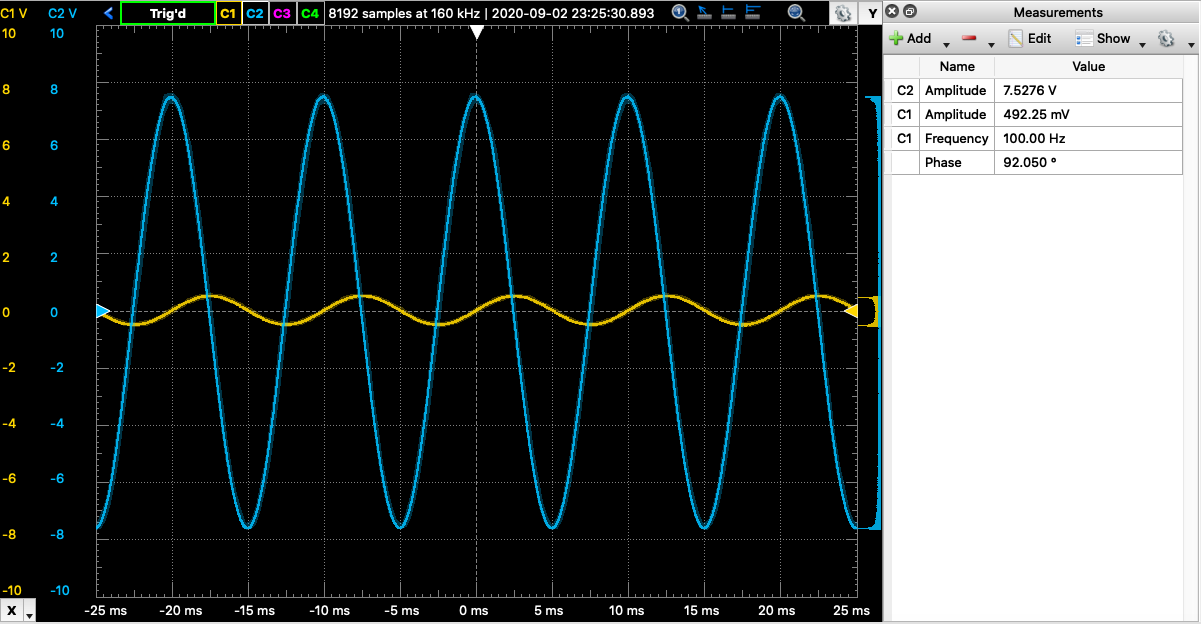
\includegraphics [scale=0.4] {../Ejercicio3-CircuitoIntegradoresyDerivadores/Imagenes/senoidal - 100.png} 
    \caption{Señal de Entrada y Salida - Frecuencia 100 Hz}
    \label{fig:emptyPlotTool}
\end{figure}

En el segundo caso, se pudo observar también el desfasaje pero la ganancia de amplitud ya reducida como era esperado.

\begin{figure}[H]
    \centering 
    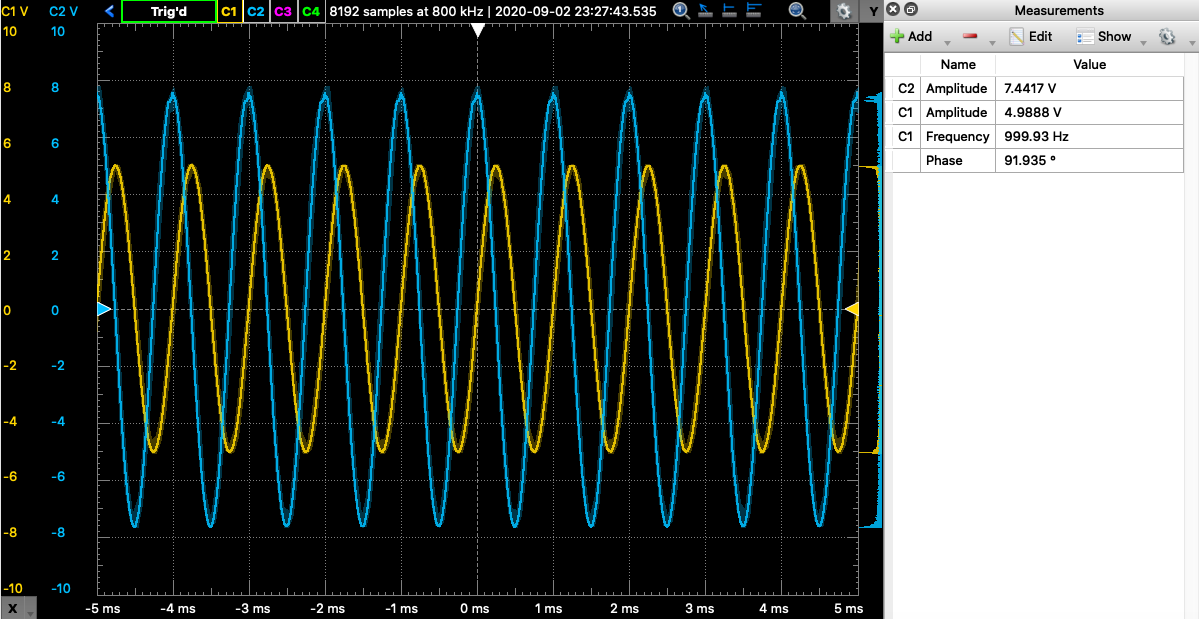
\includegraphics [scale=0.4] {../Ejercicio3-CircuitoIntegradoresyDerivadores/Imagenes/senoidal - 1000.png} 
    \caption{Señal de Entrada y Salida - Frecuencia 1.000 Hz }
    \label{fig:emptyPlotTool}
\end{figure}

Finalmente, para una frecuencia de $10$ $KHz$, la señal de salida ha reducido notablemente su amplitud en comparación a la señal de entrada. 

\begin{figure}[H]
    \centering 
    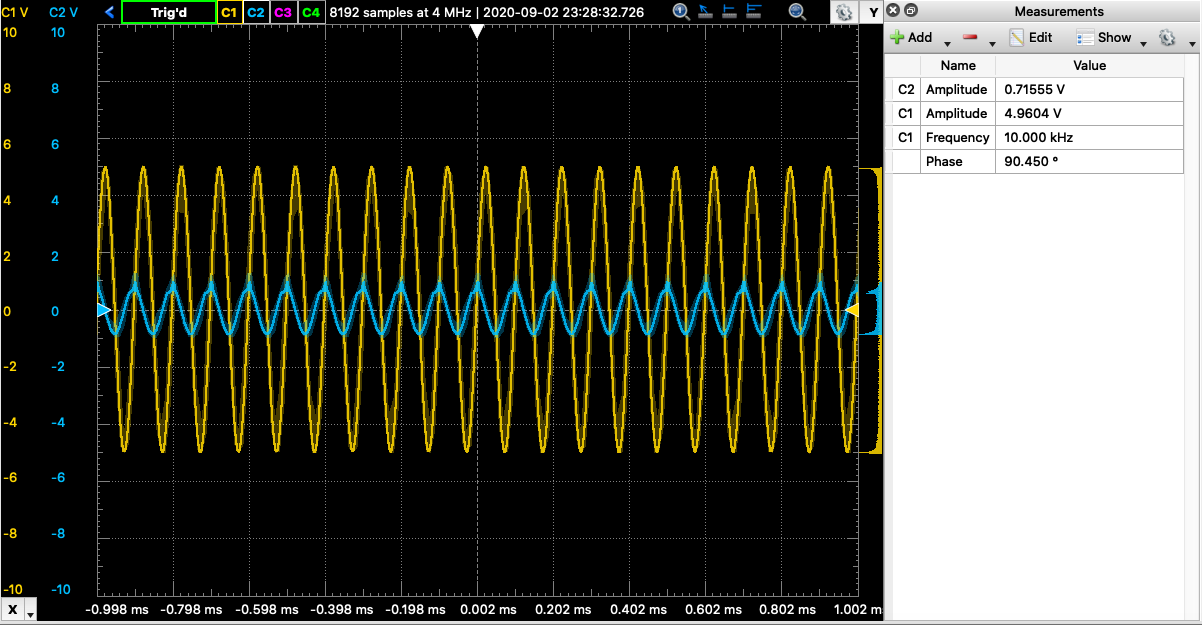
\includegraphics [scale=0.4] {../Ejercicio3-CircuitoIntegradoresyDerivadores/Imagenes/senoidal - 10000.png} 
    \caption{Señal de Entrada y Salida - Frecuencia 10.000 Hz}
    \label{fig:emptyPlotTool}
\end{figure}

Para realizar el diagrama de respuesta en frecuencia no se pudo utilizar la funcionalidad $Network$ del software $WaveForms$ ya que al realizar un barrido en frecuencia
con la misma amplitud para todos los casos, para el rango de frecuencias deseado, en las bajas frecuencias, el sistema saturía para determinada amplitud y para las frecuencias muy altas, la amplitud de la señal a la salida
está en el orden del error presentado por el osciloscopio del $Electronic$ $Explorer$ $Board$.

Se realizaron entonces mediciones manuales, variando la amplitud según la frecuencia convenientemente y resultó comparable (en las frecuencias donde se pudo realizar las mediciones)
a los modelos simulados y teórico.

\begin{figure}[H]
    \centering 
    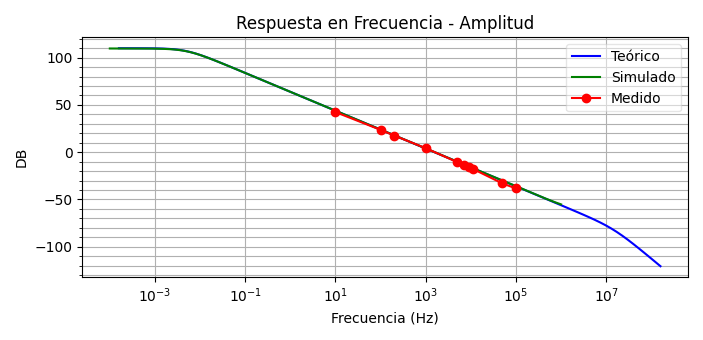
\includegraphics [scale=1] {../Ejercicio3-CircuitoIntegradoresyDerivadores/Imagenes/comparativo-integrador-amplitud.png} 
    \caption{Respuesta en Frecuencia para el Circuito Integrador Comparativo - Amplitud }
    \label{fig:emptyPlotTool}
\end{figure}

\begin{figure}[H]
    \centering 
    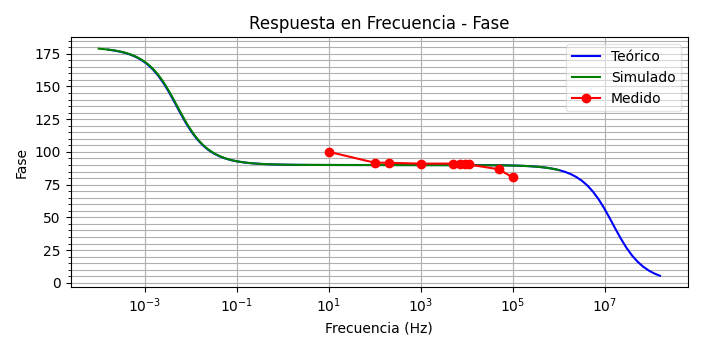
\includegraphics [scale=1] {../Ejercicio3-CircuitoIntegradoresyDerivadores/Imagenes/comparativo-integrador-fase.png} 
    \caption{Respuesta en Frecuencia para el Circuito Integrador Comparativo - Fase }
    \label{fig:emptyPlotTool}
\end{figure}

\subsubsection{Análisis de Entrada Cuadrada al Circuito Integrador}

Es importante antes de realizar el análisis para la correspondiente señal de entrada, analizar el comportamiento del capacitor en los distintos rangos de frecuencia.
A medida que la frecuencia se reduce, se pudo observar que la magnitud de la señal de salida se ve amplificada pero a su vez, la impedancia representada por el capacitor
también, ya que $X_c= \frac{1}{jwC}$. Al tener una frecuencia lo suficientemente baja, tal que la impedancia $X_c$ es lo suficientemente grande, sucederá que por el cable 
donde está conectado el capacitor no circulará corriente al tener una impedancia extremadamente grande. En otras palabras, allí habrá un circuito abierto.

Al haber un circuito abierto, el proceso de realimentación se verá interrumpido, haciendo que la diferencia mencionada en incisos anteriores que determinaba a 
$v_{out}=A_0(V^+-V^-)$ sea cada ves más grande. Esto guarda correlación con que el hecho de que si baja la frecuencia, la señal de salida se verá más y más amplificada,
y a su vez la diferencia de potencial $(V^+-V^-)$ será cada vez mayor, por estar $V^+$ conectada a tierra y por el hecho de que la retroalimentación del circuito se ve afectada
por la alta impedancia del capacitor.

Otro factor importante a tener en cuenta es que en el mundo real, los generadores de señales, incluido el generador de señales del $Electronic$ $Explorer$ $Board$ no son ideales,
por lo cual en ellos se presenta una componente de tensión continua que puede ser de mayor o menor valor. La particularidad de este circuito integrador es que amplifica las componentes 
espectrales de frecuencia baja por lo cual, dicha componente de tensión continua se verá amplificada generando un offset en la señal de salida.

Para poder realizar mediciones con mayor sencillez, se utilizado la funcionalidad $Scope$ pero conectado a la terminal $AC$ para filtrar dicha componente continua y así evitar
esa tensión de offset. 


A continuación se puede observar el comportamiento integrador del circuito en las frecuencias que así lo permiten.

\begin{figure}[H]
    \centering 
    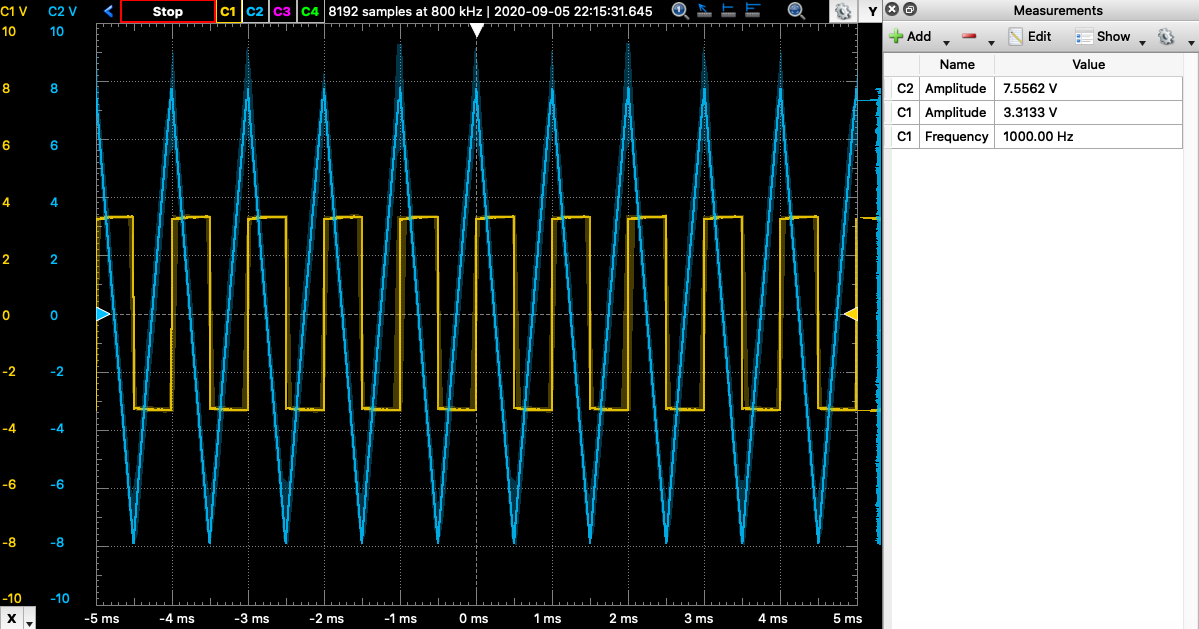
\includegraphics [scale=0.45] {../Ejercicio3-CircuitoIntegradoresyDerivadores/Imagenes/cuadrada-1000.png} 
    \caption{Señal de Entrada Cuadrada y Señal Integrada de Salida a 1000 Hz }
    \label{fig:emptyPlotTool}
\end{figure}

\begin{figure}[H]
    \centering 
    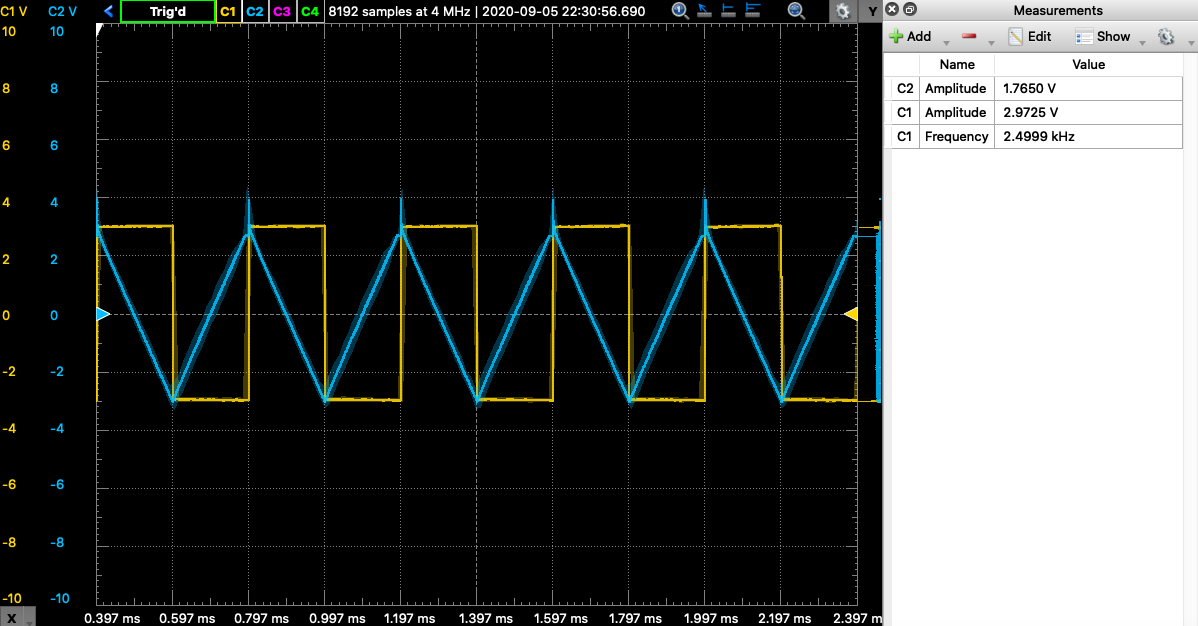
\includegraphics [scale=0.45] {../Ejercicio3-CircuitoIntegradoresyDerivadores/Imagenes/cuadrada-2500.png} 
    \caption{Señal de Entrada Cuadrada y Señal Integrada de Salida a 2500 Hz}
    \label{fig:emptyPlotTool}
\end{figure}

\begin{figure}[H]
    \centering 
    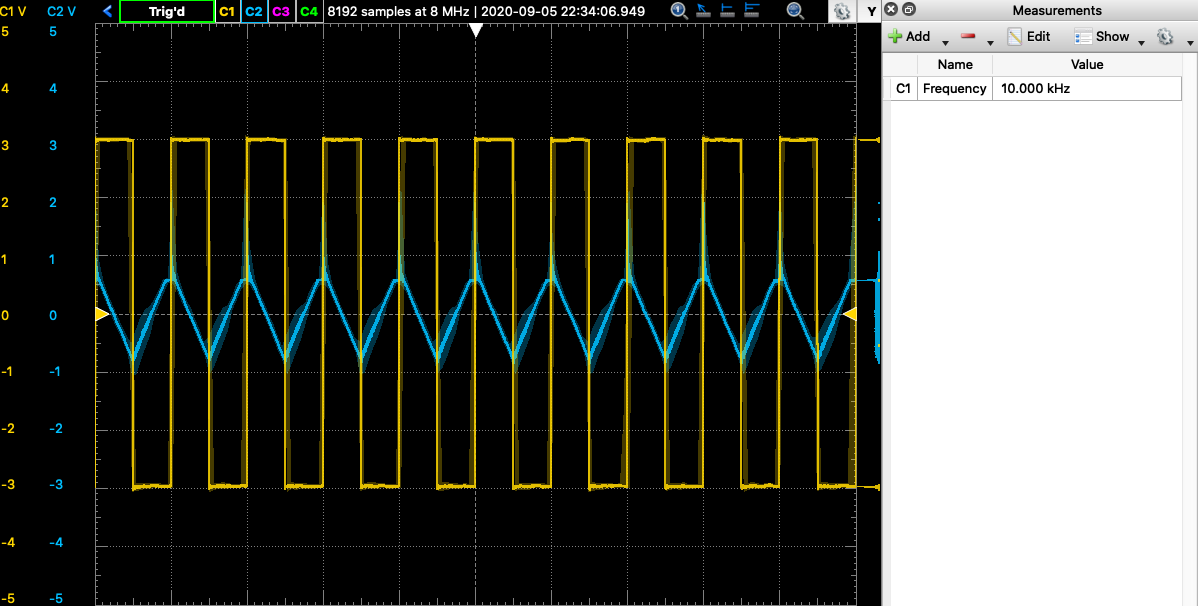
\includegraphics [scale=0.45] {../Ejercicio3-CircuitoIntegradoresyDerivadores/Imagenes/cuadrada-10000.png} 
    \caption{Señal de Entrada Cuadrada y Señal Integrada de Salida a 10.000 Hz}
    \label{fig:emptyPlotTool}
\end{figure}

En los tres casos, se puede apreciar efectivamente el comportamiento integrador del circuito. Durante los semi-ciclos donde la tensión de la señal 
de la entrada cuadrada es positiva, se puede ver la pendiente negativa en la señal triangular y la situación opuesta se presenta durante el siguiente semi-ciclo.
Además, se observa claramente que a medida que la frecuencia aumenta la amplitud de la señal triangular de salida se atenua

\subsubsection{Análisis de Impedancia de Entrada al Circuito Integrador}

Para poder calcular teóricamente la impedancia de entrada, $Z_{in}$, se utilizó el teorema de Miller tal que:

$$ V_{out}=-A_{vol}.V^-$$

Como para este caso, $K=-A_{vol}$, el circuito integrador con el amplificador operacional, queda expresado como:

\begin{figure}[H]
    \centering 
    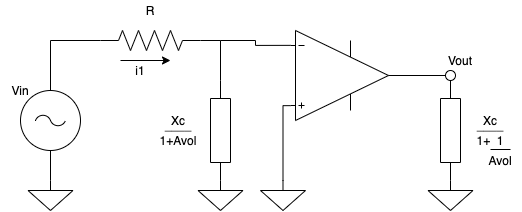
\includegraphics [scale=0.7] {../Ejercicio3-CircuitoIntegradoresyDerivadores/Imagenes/miller-integrador.png} 
    \caption{Diagrama de BODE de Fase para OPAMP comparativo }
    \label{fig:emptyPlotTool}
\end{figure}

Como nos interesa $Z_{in}=\frac{V_{in}}{i_1}$, es muy sencillo ver que a la entrada no inversora del amplificador operacional no ingresa corriente,
por lo cual utilizando la ley de tensiones de Kirchoff:

$$ V_{in} = i_1.R + i_1.\frac{X_c}{1+A_{vol}} \longrightarrow \frac{V_{in}}{i_1}= R + \frac{X_c}{1+A_{vol}} \longrightarrow Z_{in}=R+\frac{1}{SC(1+A_0)}$$

Dicha impedancia teórica puede verse expresada en las siguientes figuras en conjunto con la expresión simulada mediante $LTSpice$ para ella:

\begin{figure}[H]
    \centering 
    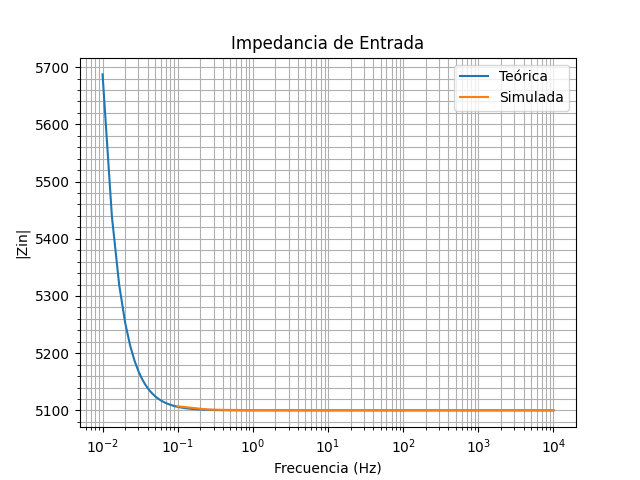
\includegraphics [scale=1] {../Ejercicio3-CircuitoIntegradoresyDerivadores/Imagenes/comparativo-integrador-zin-amplitud.png} 
    \caption{Amplitud de $Z_{in}$ en función de $f$}
    \label{fig:emptyPlotTool}
\end{figure}

\begin{figure}[H]
    \centering 
    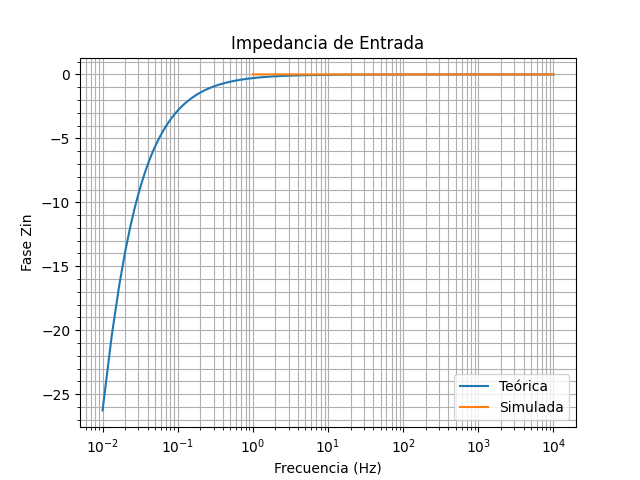
\includegraphics [scale=1] {../Ejercicio3-CircuitoIntegradoresyDerivadores/Imagenes/comparativo-integrador-zin-fase.png} 
    \caption{Fase de $Z_{in}$ en función de $f$ }
    \label{fig:emptyPlotTool}
\end{figure}

Se puede observar que a frecuencias notablemente bajas, la impedancia tiende a aumentar en magnitud ya que la componente reactiva de 
$Z_{in}$ es inversamente proporcional al valor de la frecuencia como se demostró anteriormente.
A partir de frecuencias del orden de los $mHz$, se puede observar como el efecto de la reactancia capacitiva 
se reduce, dejando unicamente la componente de la $R$. Por lo cual podemos afirmar que $Z_{in}$ es aproximadamente $R$ para esos casos, ademas del efecto que genera $A_0$.
Lo mismo se puede observar con la fase que tiende a 0, ya que la componente compleja que aporta el capacitor se ve reducida conforme aumenta la frecuencia.
Como conclusión entonces, para $f \geq 1Hz$ :

$$Z_{in} \approx R$$

\subsubsection{Compensación/Limitación del Circuito Integrador con una $R$ adicional}

Como se ha explicado previamente, para el circuito integrador con el amplificador operacional, en frecuencias bajas, se interrumpe el ciclo de retroalimentación,
ya que debido a la alta impedancia, en dichas frecuencias, del componente reactivo del circuito, se "abre" el  circuito entre los terminales donde está conectado el capacitor.

Para limitar ese efecto en las bajas frecuencias, es conveniente conectar una resistencia en paralelo al capacitor. El efecto que se logrará es que eligiendo conveniente esa resistencia,
a la que llamaremos $R_c$, se subsanará el efecto de circuito abierto entre las  terminales del capacitor a bajas frecuencias. Cuando se "abra" el circuito, la corriente de retroalimentación
aun podrá circular por dicha $R_c$ aunque a su vez, la ganancia del circuito ya no será cada vez mayor a medida que la frecuencia baja, sino que estará limitada por la relación 
$\frac{R_c}{R}$. 

Se pudo observar previamente que la ganancia tendía a $\infty$ conforme la frecuencia disminuía, ahora en ese rango de frecuencias, la ganancia estará limitada. Por ello, podemos
afirmar que el efecto de agregar la $R_c$ en paralelo al capacitor tendrá un efecto compensatorio para el efecto del capacitor en bajas frecuencias y a su vez limitador en cuanto a la 
ganancia. 

\begin{figure}[H]
    \centering 
    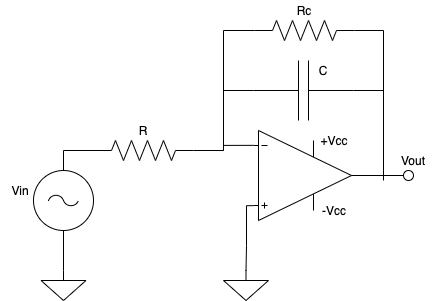
\includegraphics [scale=0.7] {../Ejercicio3-CircuitoIntegradoresyDerivadores/Imagenes/diagrama-integrador-compensado.png} 
    \caption{Diagrama del circuito integrador compensado}
    \label{fig:emptyPlotTool}
\end{figure}

Es conveniente analizar, como será el efecto de esta nueva resistencia introducida en las representaciones de las funciones transferencia para los tres
casos analizados anteriormente. Para ello, simplificaremos el diagrama definiendo a $Z=\frac{X_c.R_c}{X_c+R_c}=\frac{R_c}{SR_cC+1}$

\begin{figure}[H]
    \centering 
    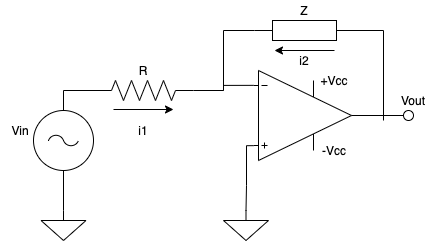
\includegraphics [scale=0.7] {../Ejercicio3-CircuitoIntegradoresyDerivadores/Imagenes/diagrama-integrador-compensado-resumido.png} 
    \caption{Diagrama del circuito integrador compensado con impedancia equivalente para $R_c$ y $C$}
    \label{fig:emptyPlotTool}
\end{figure}

Si $A_{vol} = \infty$:

\begin{itemize}
	\item $i1 = -i2$
	\item $i1 = \frac{V_{in}}{R} $
	\item $i2 = \frac{V_{out}}{Z}$
\end{itemize}

Entonces:

$$ \frac{V_{in}}{R} = - (\frac{V_{out}}{Z}) \Longrightarrow \frac{V_{out}}{V_{in}} = -\frac{Z}{R} = - \frac{R_c}{R}.\frac{1}{SCR_c+1}$$

$$ H(S) = - \frac{R_c}{R}.(\frac{1}{SCR_c+1})$$

Para el caso donde $A_{vol}$ es finito, utilizando las relaciones descriptas en el análisis sin $R_c$:

\begin{itemize}
	\item $i1 = \frac {V_{in}-V^{-}}{R} =  \frac {V_{in} + \frac{V_{out}}{A_{vol}}}{R}$
	\item $i2 = \frac {V_{out}-V^{-}}{Z} = \frac {V_{out} + \frac{V_{out}}{A_{vol}}}{Z}$
\end{itemize}

Siendo entonces:

$$ \frac {V_{in} + \frac{V_{out}}{A_{vol}}}{R} = -(\frac {V_{out} + \frac{V_{out}}{A_{vol}}}{Z})
\Longrightarrow \frac{V_{out}}{V_{in}} = \frac{-1}{(SCR_c+1)\frac{R}{R_c}(1+\frac{1}{A_{vol}})+\frac{1}{A_{vol}}} = 
-\frac{R_c}{R}\frac{1}{(SCR_c+1)(1+\frac{1}{A_{vol}})+\frac{R_c}{RA_{vol}}} $$

Por lo tanto:

$$H(S)= -\frac{R_c}{R}\frac{1}{(SCR_c+1)(1+\frac{1}{A_{vol}})+\frac{R_c}{RA_{vol}}} $$

Para finalizar este análisis, se calculará la función transferencia cuando $A_{vol}(w)$, siendo esta:

$$H(S)=-\frac{R_c}{R}\frac{1}{S^2(\frac{CR_c}{W_bA_0})+SCR_c(1+\frac{1}{A_0}+\frac{1}{W_bA_0CR_c}+\frac{1}{W_bA_0CR})+1+\frac{1}{A_0}+\frac{R_c}{RA_0}}$$

Se puede observar que para los últimos dos casos, nuevamente si $A_{vol}$ es mas y mas grande, estaremos en el caso de la ganancia ideal para el circuito compensado
por $R_c$.


Para poder conocer cuál es la $R_c$ a emplear, se buscará obtener un desfasaje de $90^o$ entre la señal de entrada y salida en frecuencias lo más baja posible.
A su vez, la ganancia de $-3Db$ por década, será buscada en esa misma frecuencia.
Contar con ambas caracteristicas implica contar con las características propias del integrador ideal. 
Para poder encontrar ese valor, y partiendo del caso ideal con la resistencia
de compensación,$ H(S) = - \frac{R_c}{R}.(\frac{1}{SCR_c+1})$, podemos observar que al introducir la resistencia $R_c$
en paralelo contamos con un nuevo polo en donde el desfasaje cambiará a $90^o$ y obtendremos la ganancia de $-3DB$ que dependerá de la frecuencia que nosotros consideremos como baja y el valor de $R_c$ empleado.
A su vez, podemos observar que para la función de transferencia ideal, contamos con la expresion de un filtro pasa-bajos pasivo como el analizado en la primera experiencia
de laboratorio. Entonces la frecuencia de corte considerada para tal puede ser expresada como:

$$f_0 = \frac{1}{2\pi R_cC}$$

Una década luego de esa frecuencia, obtendremos el comportamiento deseado propio del integrador, y a su vez la limitación en la ganancia del circuito que evitará posibles saturaciones en $V_{out}$.
Tomaremos como frecuencia de integración inicial $f=1KHz$, por lo cual para observar el efecto propio de un integrador a esta frecuencia, elegiremos como frecuencia
$f=100Hz$, ya que una década luego se observarán los efectos deseados. 

Entonces para obtener $R_c$:

$$R_c \geq \frac {1}{2\pi fC} \longrightarrow R_c \geq \frac {1}{2\pi .100.(20n)}\longrightarrow R_c \geq 79577.47 Hz$$

Entonces se ha utilizado un valor comercial de resistencia de $R_c=82KHz$. Teóricamente, se puede demostrar que en frecuencias mayores
a $970 Hz$ el sistema deberá integrar sin efectos adversos y a su vez la máxima ganancia del circuito estará denotada por $\frac {R_c}{R}$ que es el equivalente a
$24.12DB$ cuando antes a medida que las frecuencias se acercaban a $0Hz$, tendían a $110DB$. Se puede observar así nuestro efecto limitador en la ganancia.

Cabe destacar que se podría haber utilizado una $R_c$ de mayor valor, pero en ese caso la ganancia se hubiese limitado menos generando para un mayor rango de frecuencias bajas
un efecto de gran amplificación y consecuente saturación. Por ello, es que se decidió elegir el valor comercial más cercano al valor teórico obtenido.

A continuación se puede observar las funciones transferencia para los tres casos descriptos:

\begin{figure}[H]
    \centering 
    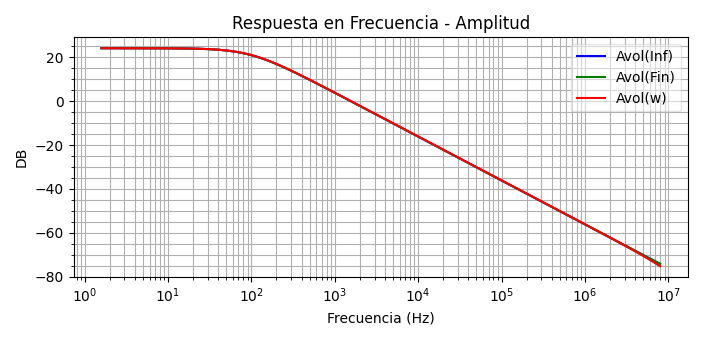
\includegraphics [scale=1] {../Ejercicio3-CircuitoIntegradoresyDerivadores/Imagenes/diagrama-bode-integrador-compensado-amplitud.png} 
    \caption{Amplitud de $Z_{in}$ en función de $f$}
    \label{fig:emptyPlotTool}
\end{figure}

\begin{figure}[H]
    \centering 
    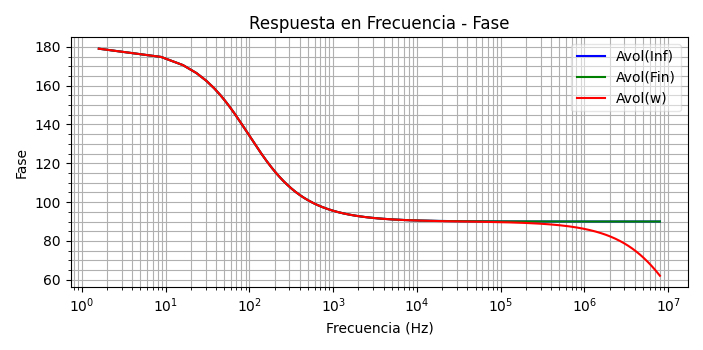
\includegraphics [scale=1] {../Ejercicio3-CircuitoIntegradoresyDerivadores/Imagenes/diagrama-bode-integrador-compensado-fase.png} 
    \caption{Fase de $Z_{in}$ en función de $f$ }
    \label{fig:emptyPlotTool}
\end{figure}

También se puede observar como la ganancia queda limitada ahora al valor de $24.12DB$ para las bajas frecuencias:

\begin{figure}[H]
    \centering 
    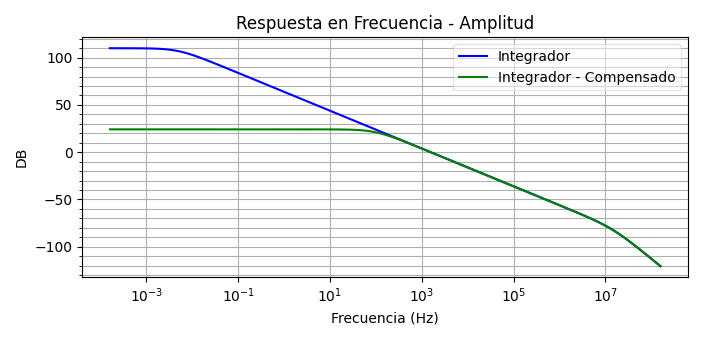
\includegraphics [scale=1] {../Ejercicio3-CircuitoIntegradoresyDerivadores/Imagenes/diagrama-bode-integrador-compensado-comparativo-amplitud.png} 
    \caption{Amplitud de $Z_{in}$ en función de $f$}
    \label{fig:emptyPlotTool}
\end{figure}

\begin{figure}[H]
    \centering 
    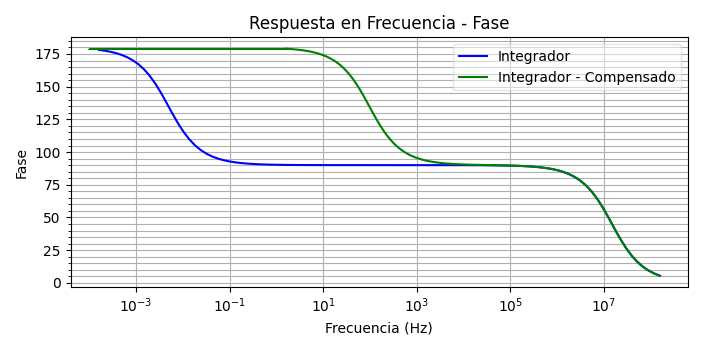
\includegraphics [scale=1] {../Ejercicio3-CircuitoIntegradoresyDerivadores/Imagenes/diagrama-bode-integrador-compensado-comparativo-fase.png} 
    \caption{Fase de $Z_{in}$ en función de $f$ }
    \label{fig:emptyPlotTool}
\end{figure}

\subsubsection{Respuesta en Frecuencia del sistema integrador compensado}

Se realizó la simulación del circuito en el software $LTSpice$, obteniendo su respuesta en frecuencia que coincide con lo obtenido teoricamente.

\begin{figure}[H]
    \centering 
    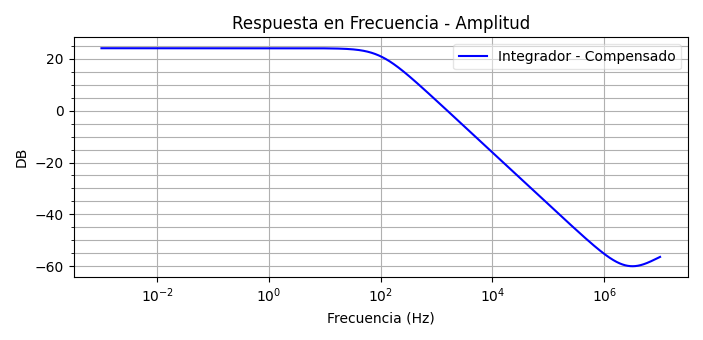
\includegraphics [scale=1] {../Ejercicio3-CircuitoIntegradoresyDerivadores/Imagenes/diagrama-bode-integrador-simulado-compensado-amplitud.png} 
    \caption{Amplitud de $Z_{in}$ en función de $f$}
    \label{fig:emptyPlotTool}
\end{figure}

\begin{figure}[H]
    \centering 
    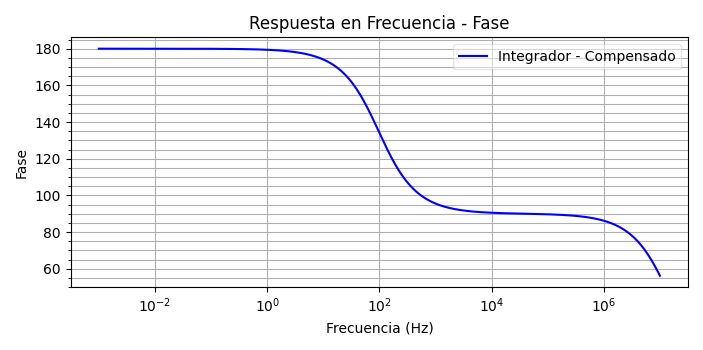
\includegraphics [scale=1] {../Ejercicio3-CircuitoIntegradoresyDerivadores/Imagenes/diagrama-bode-integrador-simulado-compensado-fase.png} 
    \caption{Fase de $Z_{in}$ en función de $f$ }
    \label{fig:emptyPlotTool}
\end{figure}

Además de ello, se realizó la medición de la respuesta en frecuencia utilizando el $Electronic$ $Explorer$ $Board$. Es importante mencionar
que en este caso debido a la limitación en la ganancia, se pudieron realizar mediciones en frecuencias donde antes no era posible por la alta ganancia
en dichas frecuencias que generaban una saturación aun en valores pequeños de amplitud.

\begin{figure}[H]
    \centering 
    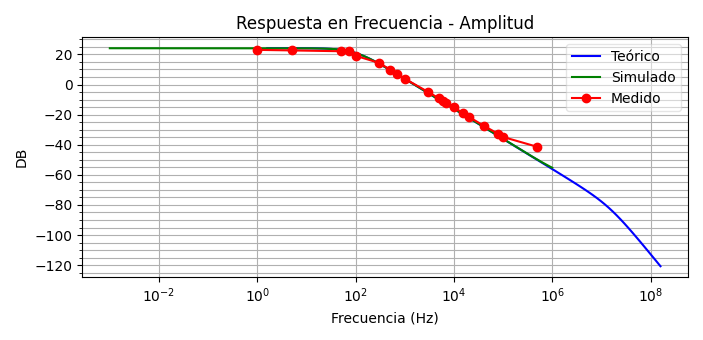
\includegraphics [scale=1] {../Ejercicio3-CircuitoIntegradoresyDerivadores/Imagenes/transferencia-comparativo-todo-amplitud.png} 
    \caption{Amplitud de $Z_{in}$ en función de $f$}
    \label{fig:emptyPlotTool}
\end{figure}

\begin{figure}[H]
    \centering 
    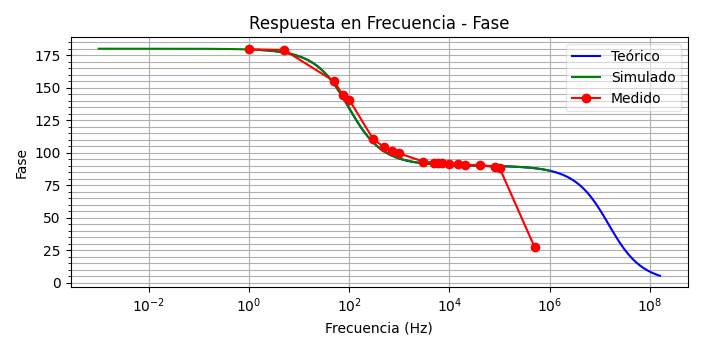
\includegraphics [scale=1] {../Ejercicio3-CircuitoIntegradoresyDerivadores/Imagenes/transferencia-comparativo-todo-fase.png} 
    \caption{Fase de $Z_{in}$ en función de $f$ }
    \label{fig:emptyPlotTool}
\end{figure}

Se puede observar que tantos el modelo teórico, simulado y experimental coinciden en su comportamiento. Se puede notar también que
en frecuencias del orden de $1MHz$, al ser tanta la atenuación no es posible medir con precisión la señal de salida.

